\section{Функциональный и интерактивный интерфейс Unix Taskbook}

\subsection{Запуск задачника}

\subsubsection{Компиляция динамических библиотек}

Чтобы получить динамические библиотеки, которые могут быть загружены ядром, мы 
сначала должны скомпилировать файлы классов отдельных динамических библиотек, которые мы написали.

Но когда количество динамических библиотек растет, компилировать их по отдельности и 
вручную может быть хлопотно. Поэтому мы написали файл runlib.cmd для компиляции всех 
необходимых динамических библиотек в одном файле.

\centerline{\textbf{runlib.cmd}}

\lstset{language=bash}
\begin{lstlisting}
#!/bin/bash
if ! [ -d ~/utblib ]; then mkdir ~/utblib; fi
g++ -fPIC utbDir.cpp utilities.cpp -shared -o ~/utblib/libutbDir.so
g++ -fPIC utbFile.cpp utilities.cpp -shared -o ~/utblib/libutbFile.so
g++ -fPIC utbText.cpp utilities.cpp -shared -o ~/utblib/libutbText.so
g++ -fPIC utbShell.cpp utilities.cpp -shared -o ~/utblib/libutbShell.so
g++ -fPIC utbBegin.cpp pt4utilities.cpp udata.cpp uprint.cpp -shared -o ~/utblib/libutbBegin.so
g++ -fPIC utbMPI1Proc.cpp pt4utilities.cpp udata.cpp uprint.cpp -shared -o ~/utblib/libutbMPI1Proc.so
g++ -fPIC utbMPI2Send.cpp pt4utilities.cpp udata.cpp uprint.cpp -shared -o ~/utblib/libutbMPI2Send.so
g++ -fPIC utbMPI3Coll.cpp pt4utilities.cpp udata.cpp uprint.cpp -shared -o ~/utblib/libutbMPI3Coll.so
g++ -fPIC utbMPI4Type.cpp pt4utilities.cpp udata.cpp uprint.cpp -shared -o ~/utblib/libutbMPI4Type.so
g++ -fPIC utbMPI5Comm.cpp pt4utilities.cpp udata.cpp uprint.cpp -shared -o ~/utblib/libutbMPI5Comm.so
\end{lstlisting}

Перед компиляцией мы проверим, существует ли каталог utblib в каталоге текущего
 пользователя, если нет, то он будет создан автоматически, и все динамические
  библиотеки будут автоматически сохранены в этом каталоге после компиляции, чтобы 
  мы могли легко управлять и находить динамические библиотеки в будущем.

Чтобы запустить cmd-файл, нам нужно убедиться, что все файлы классов динамической 
библиотеки находятся в том же каталоге, что и cmd-файл, а затем выполнить команду \textbf{./runlib.cmd}

\subsubsection{Компиляция ядра}

Следующим шагом будет компиляция для получения исполняемого файла unixTaskbook.

Из-за большого количества файлов и параметров компиляции, необходимых для 
компиляции, мы написали файл run.cmd, чтобы упростить команду компиляции.

\centerline{\textbf{run.cmd}}

\lstset{language=bash}
\begin{lstlisting}
#!/bin/bash
g++ main.cpp unixTaskbook.cpp utilities.cpp tasklib.cpp error.cpp service.cpp -o unixTaskbook -ldl
\end{lstlisting}

Чтобы запустить cmd-файл, нам нужно убедиться, что все файлы классов динамической 
библиотеки находятся в том же каталоге, что и cmd-файл, а затем выполнить команду \textbf{./run.cmd}

\subsubsection{Выполнение тестов}

После компиляции всех необходимых файлов, чтобы начать использовать unixTaskbook, нам 
нужно написать тестовый файл, выбрать задачу, которую мы хотим выполнить, создать .c файл 
с именем задачи и передать имя файла в качестве параметра выполнения в файл runtest.cmd, и 
мы можем начать выполнение теста.

Например, мы хотим выполнить задачу 7 в группе задач MPI1Proc: 
\\ \textbf{./runtest.cmd MPI1Proc7.c}

\centerline{\textbf{runtest.cmd}}

\lstset{language=bash}
\begin{lstlisting}
#!/bin/bash
LD_LIBRARY_PATH=~/utblib
export LD_LIBRARY_PATH
../unixTaskbook -t $1
\end{lstlisting}

В файле runtest.cmd мы экспортируем переменную LD\_LIBRARY\_PATH, 
которая сообщает компилятору, где находятся все динамические библиотеки.

\subsection{Примеры использования разработанных групп заданий}

\begin{figure}[htbp]%
    \centering
    \subfloat[right solution]{%第一个子图
    \label{right}%子图标签
    
\includegraphics[width=0.8\linewidth]{images/right.jpg}%子图文件名
    }\\%换行
    \subfloat[wrong solution]{%第二个子图
    \label{wrong}%子图标签
    
\includegraphics[width=0.8\linewidth]{images/wrong.jpg}%子图文件名
    }\\%换行
    \subfloat[invalid data]{%第三个子图
    \label{invalid}%子图标签
    
\includegraphics[width=0.8\linewidth]{images/invalid.jpg}%子图文件名
    }\\%换行
    \subfloat[superfluous data]{%第四个子图
    \label{superfluous}%子图标签
    
\includegraphics[width=0.8\linewidth]{images/superfluous.jpg}%子图文件名
    }\\
    \subfloat[lack of data]{%第五个子图
    \label{lack}%子图标签
    
\includegraphics[width=0.8\linewidth]{images/notoutput.jpg}%子图文件名
    }
    \caption{Task info.}%总标题
    \label{task info}%总标签
\end{figure}

\begin{itemize} 
    \item Если результаты всех процессов верны, на экране появляется \textbf{Right solution} \ref{right};
    \item Если выход процесса не соответствует правильному ответу, на экране появляется \textbf{Wrong solution} \ref{wrong}, где число в начале обозначает номер процесса;
    \item Если процесс пытается ввести или вывести данные, которые не соответствуют запрошенному типу, на экране появляется сообщение \textbf{Invalid type is used for an input/output data item} \ref{invalid}, где число в начале обозначает номер процесса;
    \item Если процесс пытается ввести или вывести лишние данные, на экране появляется \textbf{An attempt to input/output superfluous data} \ref{superfluous}, где число в начале обозначает номер процесса;
    \item Если данные в процессе не вводятся или не выводятся, на экране появляется \textbf{Data are not output/input} или \textbf{Some required data are not output/input}, где число в начале обозначает номер процесса;
\end{itemize}

\subsubsection{MPI1Proc7}

\begin{figure}[htbp]%
    \centering
    \subfloat[Правильно]{%第一个子图
    \label{righ solution MPI1Proc7}%子图标签
    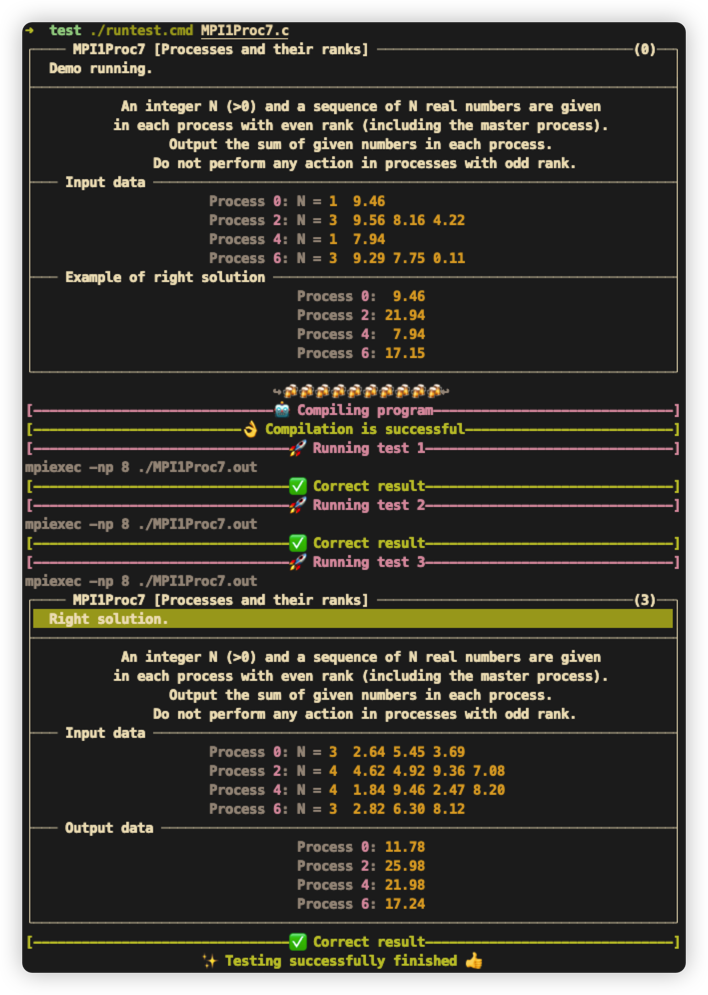
\includegraphics[width=0.5\linewidth]{images/mpi1_eg_r.jpg}%子图文件名
    }\hfill%水平间距
    \subfloat[Неисправность]{%第二个子图
    \label{wrong solution MPI1Proc7}%子图标签
    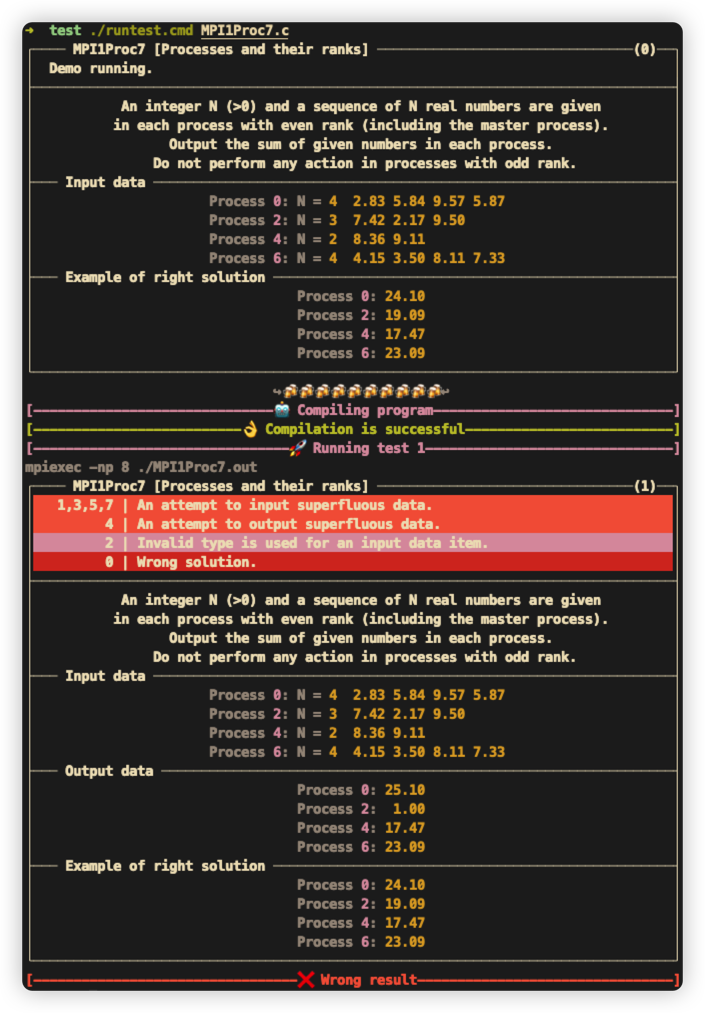
\includegraphics[width=0.5\linewidth]{images/mpi1_eg_w.jpg}%子图文件名
    }
    \caption{MPI1Proc.}%总标题
    \label{mpi1proc}%总标签
\end{figure}

% \begin{figure}[htbp]%
%     \centering
%     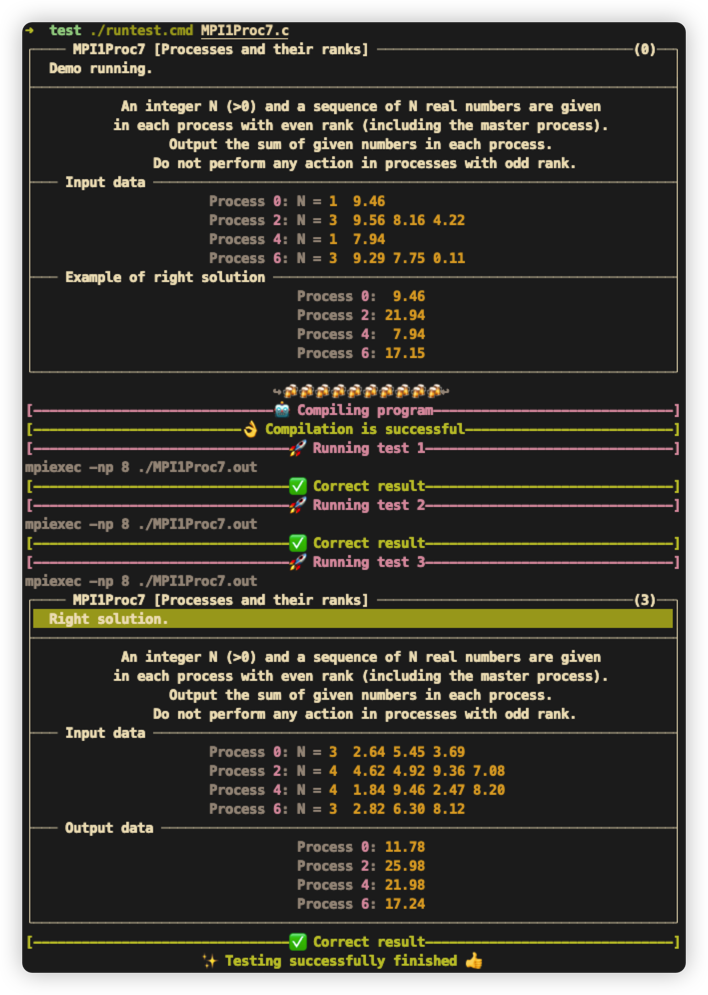
\includegraphics[width=0.6\linewidth]{images/mpi1_eg_r.jpg}%子图文件名
%     \caption{MPI1Proc.}%总标题
%     \label{mpi1proc}%总标签
% \end{figure}

\lstset{language=c++}
\begin{lstlisting}
#include "ut1.h"
int main()
{
    MPI_Init(NULL, NULL);
    int rank, size;
    MPI_Comm_size(MPI_COMM_WORLD, &size);
    MPI_Comm_rank(MPI_COMM_WORLD, &rank);
    if (!(rank % 2)) {
        int n;
        double num;
        double sum = 0;
        GetN(&n);
        for (int i = 0; i < n; ++i) {
            GetD(&num);
            sum += num;
        }
        PutD(sum);
    }
    MPI_Finalize();
}
\end{lstlisting}

Код выводит правильный ответ \ref{righ solution MPI1Proc7}.

\lstset{language=c++}
\begin{lstlisting}
#include "ut1.h"
int main()
{
    MPI_Init(NULL, NULL);
    int rank, size;
    MPI_Comm_size(MPI_COMM_WORLD, &size);
    MPI_Comm_rank(MPI_COMM_WORLD, &rank);
    if (rank == 0) {
        int n;
        double num;
        double sum = 0;
        GetN(&n);
        for (int i = 0; i < n; ++i) {
            GetD(&num);
            sum += num;
        }
        PutD(sum + 1);
    }

    if (rank == 1) {
        int n;
        double num;
        double sum = 0;
        GetN(&n);
        for (int i = 0; i < n; ++i) {
            sum += num;
        }
        PutD(sum);
    }

    if (rank == 2) {
        int n;
        int num;
        double sum = 0;
        GetN(&n);
        for (int i = 0; i < n; ++i) {
            GetN(&num);
            sum += num;
        }
        PutD(sum + 1);
    }

    if (rank == 3) {
        int n;
        double num;
        double sum = 0;
        GetN(&n);
        GetN(&n);
        for (int i = 0; i < n; ++i) {
            GetD(&num);
            sum += num;
        }
        PutD(sum);
    }

    if (rank == 4) {
        int n;
        double num;
        double sum = 0;
        GetN(&n);
        for (int i = 0; i < n; ++i) {
            GetD(&num);
            sum += num;
        }
        PutD(sum);
        PutD(sum);
    }

    if (rank == 5) {
        int n;
        double num;
        double sum = 0;
        GetN(&n);
        for (int i = 0; i < n; ++i) {
            GetD(&num);
            sum += num;
        }
        PutD(sum);
    }

    if (rank == 6) {
        int n;
        double num;
        double sum = 0;
        GetN(&n);
        for (int i = 0; i < n; ++i) {
            GetD(&num);
            sum += num;
        }
        PutD(sum);
    }

    if (rank == 7) {
        int n;
        double num;
        double sum = 0;
        GetN(&n);
        for (int i = 0; i < n; ++i) {
            GetD(&num);
            sum += num;
        }
        PutD(sum);
    }

    
    MPI_Finalize();
}
\end{lstlisting}

Мы намеренно создали ряд ошибок в различных процессах, в результате чего в конце было выведено несколько различных сообщений об ошибках \ref{wrong solution MPI1Proc7}.

\newpage

\subsubsection{MPI2Send1}

\begin{figure}[htbp]%
    \centering
    \subfloat[Правильно]{%第一个子图
    \label{righ solution MPI2Send1}%子图标签
    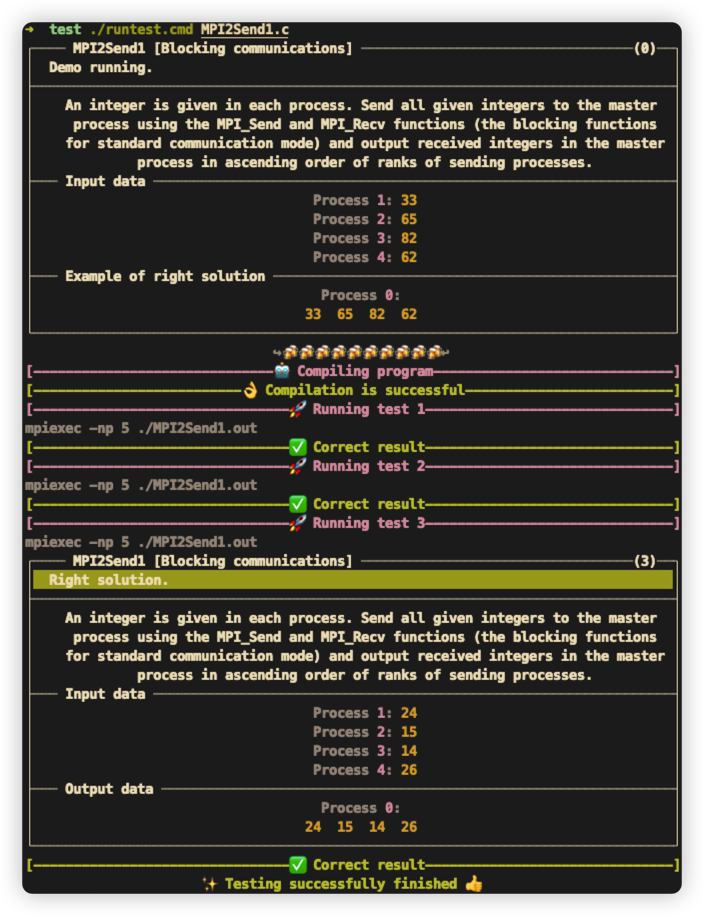
\includegraphics[width=0.5\linewidth]{images/mpi2_eg_r.jpg}%子图文件名
    }\hfill%水平间距
    \subfloat[Неисправность]{%第二个子图
    \label{wrong solution MPI2Send1}%子图标签
    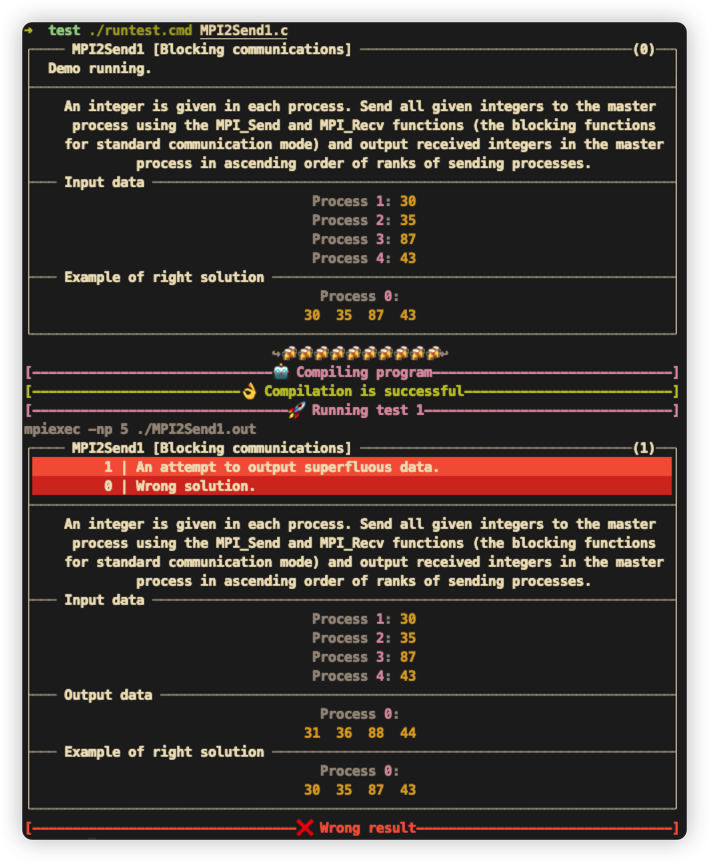
\includegraphics[width=0.5\linewidth]{images/mpi2_eg_w.jpg}%子图文件名
    }
    \caption{MPI2Send.}%总标题
    \label{mpi2send}%总标签
\end{figure}

\lstset{language=c++}
\begin{lstlisting}
#include "ut1.h"
int main()
{
    MPI_Init(NULL, NULL);
    int rank, size;
    MPI_Comm_size(MPI_COMM_WORLD, &size);
    MPI_Comm_rank(MPI_COMM_WORLD, &rank);
    int n;

    if (!rank) {
        for (int i = 1; i < size; ++i) {
            MPI_Recv(&n, 1, MPI_INT, i, 0, MPI_COMM_WORLD, MPI_STATUS_IGNORE);
            PutN(n);
        }
    }
    else {
        GetN(&n);
        MPI_Send(&n, 1, MPI_INT, 0, 0, MPI_COMM_WORLD);
    }
	MPI_Finalize();
}
\end{lstlisting}

Код выводит правильный ответ \ref{righ solution MPI2Send1}.

\lstset{language=c++}
\begin{lstlisting}
#include "ut1.h"
int main()
{
    MPI_Init(NULL, NULL);
    int rank, size;
    MPI_Comm_size(MPI_COMM_WORLD, &size);
    MPI_Comm_rank(MPI_COMM_WORLD, &rank);
    int n;

    if (!rank) {
        for (int i = 1; i < size; ++i) {
            MPI_Recv(&n, 1, MPI_INT, i, 0, MPI_COMM_WORLD, MPI_STATUS_IGNORE);
            PutN(n + 1);
        }
    }
    else {
        GetN(&n);
        MPI_Send(&n, 1, MPI_INT, 0, 0, MPI_COMM_WORLD);
        if (rank == 1)
            PutN(n);
    }
	MPI_Finalize();
}
\end{lstlisting}

Мы намеренно создали ряд ошибок в различных процессах, в результате чего в конце было выведено несколько различных сообщений об ошибках \ref{wrong solution MPI2Send1}.

\newpage

\subsubsection{MPI3Coll2}

\begin{figure}[htbp]%
    \centering
    \subfloat[Правильно]{%第一个子图
    \label{righ solution MPI3Coll2}%子图标签
    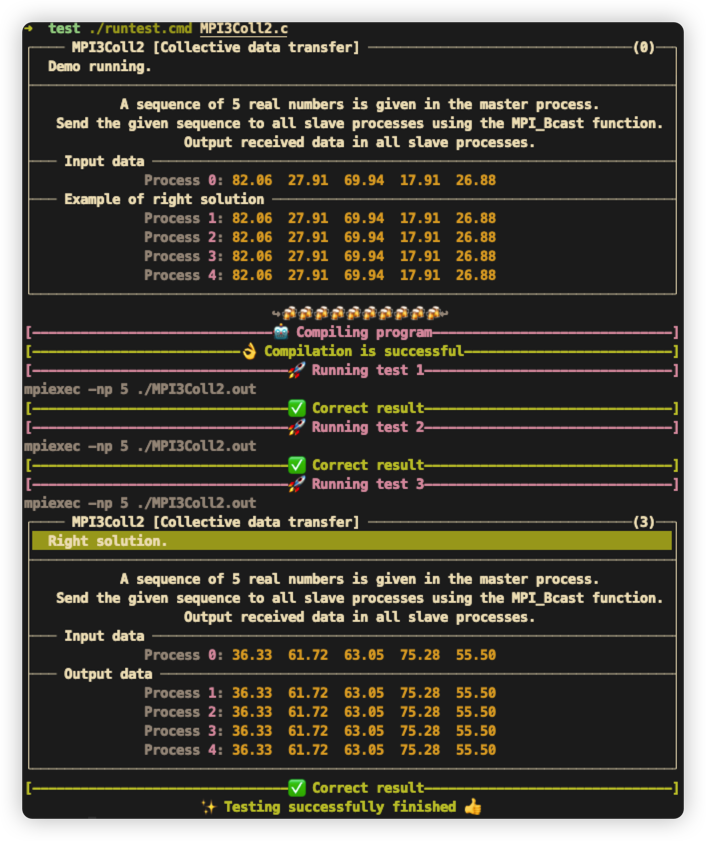
\includegraphics[width=0.5\linewidth]{images/mpi3_eg_r.jpg}%子图文件名
    }\hfill%水平间距
    \subfloat[Неисправность]{%第二个子图
    \label{wrong solution MPI3Coll2}%子图标签
    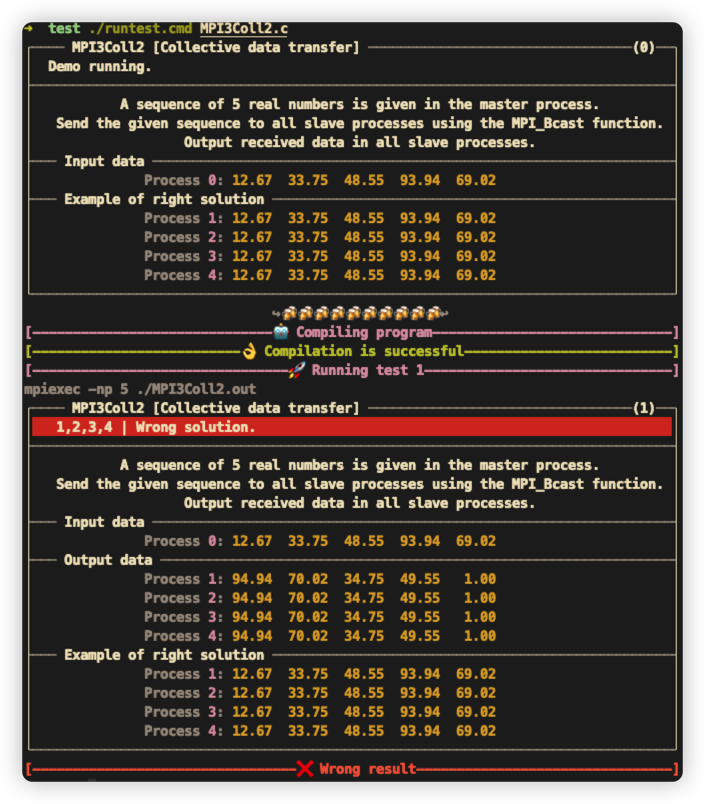
\includegraphics[width=0.5\linewidth]{images/mpi3_eg_w.jpg}%子图文件名
    }
    \caption{MPI3Coll.}%总标题
    \label{mpi3coll}%总标签
\end{figure}

\lstset{language=c++}
\begin{lstlisting}
#include "ut1.h"
int main()
{
	MPI_Init(NULL, NULL);
	int rank, size;
	MPI_Comm_size(MPI_COMM_WORLD, &size);
	MPI_Comm_rank(MPI_COMM_WORLD, &rank);
	double numbers[5];
	if (rank == 0)
		for (int i = 0; i < 5; ++i)
			GetD(&numbers[i]);
	MPI_Bcast(&numbers, 5, MPI_DOUBLE, rank, MPI_COMM_WORLD);
	if (rank != 0)
		for (int i = 0; i < 5; ++i)
			PutD(numbers[i]);

	MPI_Finalize();
}
\end{lstlisting}

Код выводит правильный ответ \ref{righ solution MPI3Coll2}.

\lstset{language=c++}
\begin{lstlisting}
#include "ut1.h"
int main()
{
	MPI_Init(NULL, NULL);
	int rank, size;
	MPI_Comm_size(MPI_COMM_WORLD, &size);
	MPI_Comm_rank(MPI_COMM_WORLD, &rank);
	double numbers[5];
	if (rank == 0)
		for (int i = 0; i < 5; ++i)
			GetD(&numbers[(i+1)%4]);
	MPI_Bcast(&numbers, 5, MPI_DOUBLE, rank, MPI_COMM_WORLD);
	if (rank != 0)
		for (int i = 0; i < 5; ++i)
			PutD(numbers[i]+1);

	MPI_Finalize();
}
\end{lstlisting}

Мы намеренно создали ряд ошибок в различных процессах, в результате чего в конце было выведено несколько различных сообщений об ошибках \ref{wrong solution MPI3Coll2}.

\newpage

\subsubsection{MPI4Type1}

\begin{figure}[htbp]%
    \centering
    \subfloat[Правильно]{%第一个子图
    \label{righ solution MPI4Type1}%子图标签
    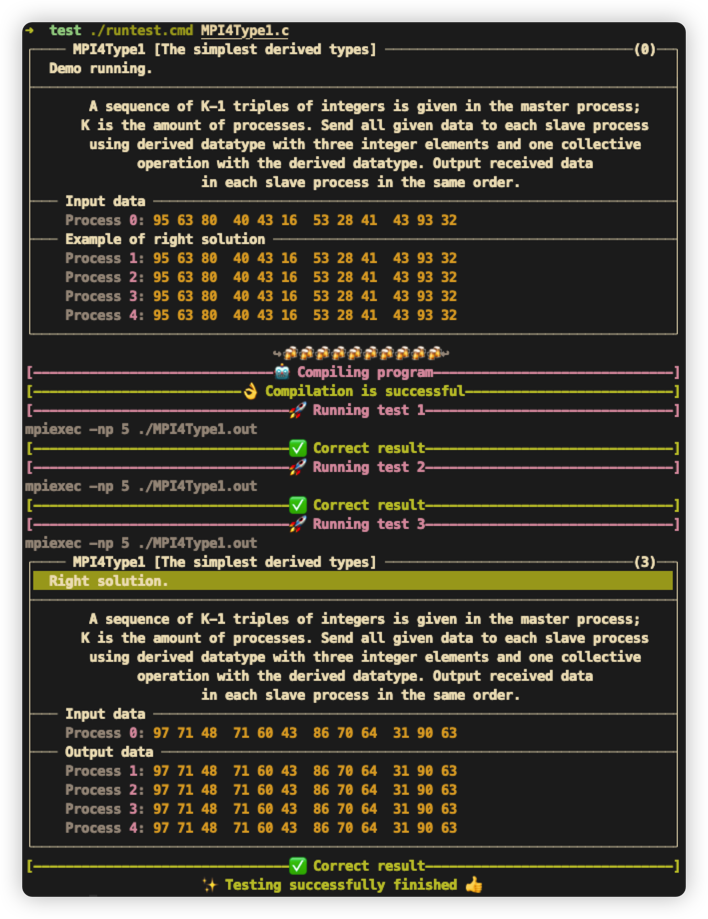
\includegraphics[width=0.5\linewidth]{images/mpi4_eg_r.jpg}%子图文件名
    }\hfill%水平间距
    \subfloat[Неисправность]{%第二个子图
    \label{wrong solution MPI4Type1}%子图标签
    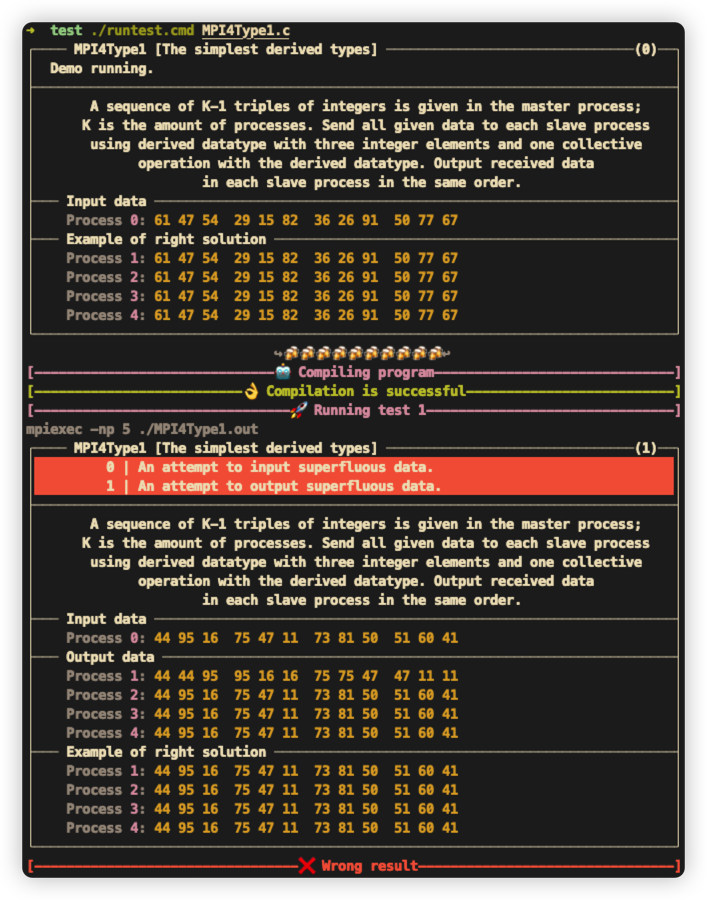
\includegraphics[width=0.5\linewidth]{images/mpi4_eg_w.jpg}%子图文件名
    }
    \caption{MPI4Type.}%总标题
    \label{mpi4type}%总标签
\end{figure}

\lstset{language=c++}
\begin{lstlisting}
#include "ut1.h"
int main()
{
	MPI_Init(NULL, NULL);
	int rank, size;
	MPI_Comm_size(MPI_COMM_WORLD, &size);
	MPI_Comm_rank(MPI_COMM_WORLD, &rank);

	MPI_Datatype newtype;
	MPI_Type_contiguous(3, MPI_INT, &newtype);
	MPI_Type_commit(&newtype);

	int *numbers = (int*)malloc((size - 1) * 3 * sizeof(int));

	if (rank == 0)
		for (int i = 0; i < (size - 1) * 3; ++i)
			GetN(&numbers[i]);

	MPI_Bcast(numbers, size - 1, newtype, 0, MPI_COMM_WORLD);

	if (rank != 0)
		for (int i = 0; i < (size - 1) * 3; ++i)
			PutN(numbers[i]);

	MPI_Type_free(&newtype);
	free(numbers);
	numbers = NULL;
	MPI_Finalize();
}
\end{lstlisting}

Код выводит правильный ответ \ref{righ solution MPI4Type1}.

\lstset{language=c++}
\begin{lstlisting}
#include "ut1.h"
int main()
{
	MPI_Init(NULL, NULL);
	int rank, size;
	MPI_Comm_size(MPI_COMM_WORLD, &size);
	MPI_Comm_rank(MPI_COMM_WORLD, &rank);

	MPI_Datatype newtype;
	MPI_Type_contiguous(3, MPI_INT, &newtype);
	MPI_Type_commit(&newtype);

	int *numbers = (int*)malloc((size - 1) * 3 * sizeof(int));

	if (rank == 0)
		for (int i = 0; i < (size - 1) * 3 + 1; ++i)
			GetN(&numbers[i]);

	MPI_Bcast(numbers, size - 1, newtype, 0, MPI_COMM_WORLD);

	if (rank != 0)
		for (int i = 0; i < (size - 1) * 3; ++i)
		{
			PutN(numbers[i]);
			if (rank == 1)
				PutN(numbers[i]);
		}

	MPI_Type_free(&newtype);
	free(numbers);
	numbers = NULL;
	MPI_Finalize();
}
\end{lstlisting}

Мы намеренно создали ряд ошибок в различных процессах, в результате чего в конце было выведено несколько различных сообщений об ошибках \ref{wrong solution MPI4Type1}.

\newpage

\subsubsection{MPI5Comm4}

\begin{figure}[htbp]%
    \centering
    \subfloat[Правильно]{%第一个子图
    \label{righ solution MPI5Comm4}%子图标签
    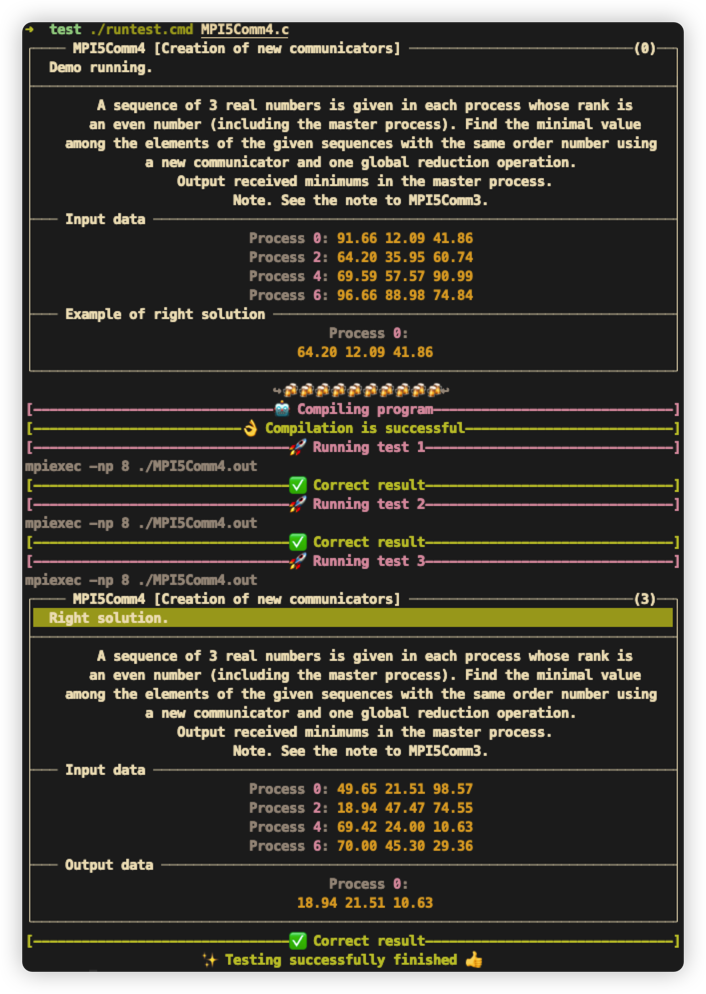
\includegraphics[width=0.5\linewidth]{images/mpi5_eg_r.jpg}%子图文件名
    }\hfill%水平间距
    \subfloat[Неисправность]{%第二个子图
    \label{wrong solution MPI5Comm4}%子图标签
    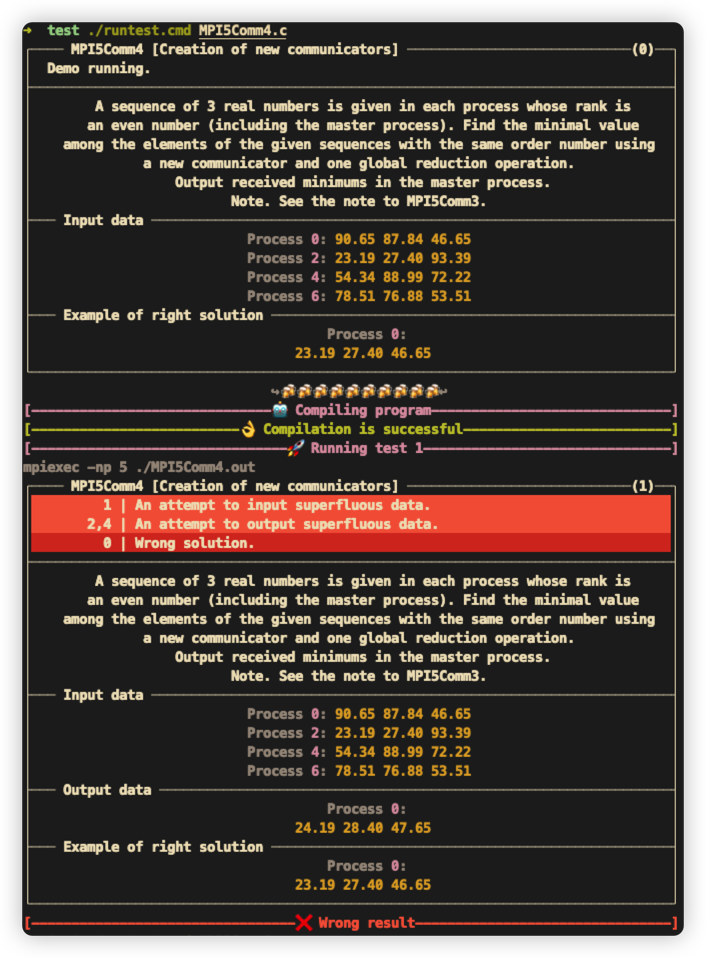
\includegraphics[width=0.5\linewidth]{images/mpi5_eg_w.jpg}%子图文件名
    }
    \caption{MPI5Comm.}%总标题
    \label{mpi5comm}%总标签
\end{figure}

\lstset{language=c++}
\begin{lstlisting}
#include "ut1.h"
int main()
{
	MPI_Init(NULL, NULL);
	int rank, size;
	MPI_Comm_rank(MPI_COMM_WORLD, &rank);
	MPI_Comm_size(MPI_COMM_WORLD, &size);

	MPI_Group even;
	MPI_Comm even_comm;
	int color = rank % 2;
	MPI_Comm_split(MPI_COMM_WORLD, color, rank, &even_comm);

	if (rank % 2 == 0)
	{
		double nums[3];
		for (int i = 0; i < 3; ++i)
			GetD(&nums[i]);
		double result[3];
		MPI_Reduce(nums, result, 3, MPI_DOUBLE, MPI_MIN, 0, even_comm);
		if (rank == 0)
			for (int i = 0; i < 3; ++i)
				PutD(result[i]);
	}
	MPI_Finalize();
}
\end{lstlisting}

Код выводит правильный ответ \ref{righ solution MPI5Comm4}.

\lstset{language=c++}
\begin{lstlisting}
#include "ut1.h"
int main()
{
	MPI_Init(NULL, NULL);
	int rank, size;
	MPI_Comm_rank(MPI_COMM_WORLD, &rank);
	MPI_Comm_size(MPI_COMM_WORLD, &size);

	MPI_Group even;
	MPI_Comm even_comm;
	int color = rank % 2;
	MPI_Comm_split(MPI_COMM_WORLD, color, rank, &even_comm);

	if (rank == 1)
	{
		double a;
		GetD(&a);
	}
	if (rank % 2 == 0)
	{
		double nums[3];
		for (int i = 0; i < 3; ++i)
			GetD(&nums[i]);
		if (rank != 0)
			PutD(nums[0]);
		double result[3];
		MPI_Reduce(nums, result, 3, MPI_DOUBLE, MPI_MIN, 0, even_comm);
		if (rank == 0)
			for (int i = 0; i < 3; ++i)
				PutD(result[i] + 1);
	}
	MPI_Finalize();
}
\end{lstlisting}

Мы намеренно создали ряд ошибок в различных процессах, в результате чего в конце было выведено несколько различных сообщений об ошибках \ref{wrong solution MPI5Comm4}.

\newpage
